\documentclass[runningheads,a4paper]{llncs}

\usepackage{amssymb}
\setcounter{tocdepth}{3}
\usepackage{graphicx}
\usepackage{url}
\usepackage{epsfig}


\urldef{\mailalex}\path|{alexander.toschev@gmail.com}|
\urldef{\mailmax}\path|{max.talanov@gmail.com}|
\urldef{\mailand}\path|{andrey.krekhov@ts.fujitsu.com}|

\begin{document}

\mainmatter

\title{Thinking Lifecycle as an implementation of machine understanding in software maintenance domain}

\titlerunning{Thinking Lifecycle implementation in ITSM}

\author{Alexander Toschev\inst{1} \and Maxim Talanov\inst{2} \and Andrey Krekhov\inst{3}}
\institute{Kazan State University, Chebotarev Research Institute of Mathematics and Mechanics\\
Universitetskaya 17, 420008 Kazan, Russia\\
\mailalex\\
\and
Fujitsu GDC Russia, Kazan, Russia\\
\mailmax\\
\and
Fujitsu GDC Russia,\\
Sibirskii trakt 34, 420029 Kazan, Russia\\
\mailand\\
}


\maketitle

\begin{abstract}
IT maintenance domain is wide and contains a lot of tools that helps to solve a lot of every-day problems. IT maintenance also has a lot of primitive incidents that seems to be easy to automate. However there is still the gap occupied by human specialist understanding and decision making as well as implementation even primitive incidents. But one of the key to understanding input request is the human being thinking processes: correlation, simulation, annotation. Using this model it is much easy to parse incoming request in natural language. In 2006 Marvin Minsky has published his book \cite{minsk} which was our inspiration and the base of implementation described below.

\keywords{AI, machine understanding, it outsourcing}

\end{abstract}

\section{Introduction}
This implementation contains machine understanding model based on thinking model because human understanding is also based on human thinking. \\
In 2006 year Marvin Minsky has published his book “The Emotion Machine” where he describes model of human thinking dividing all actions into 3 categories:

\begin{enumerate}
 \item Critic
 \item Selector
 \item Way To Think
\end{enumerate}

\subsection{Critic}
Critic could be understood as probabilistic predicate. In real world when human faces with the problem several critics are activated. In ITSM model\footnote{ITSM - IT Service Management - model of IT services} there is Direct Instruction Critic (will be described below) which activates when direct instruction incident has been received. After activating critic returns Selector.
For example:

\begin{enumerate}
 \item Learned Reactive Critics.
 \item Deliberative Critics.
 \item Reflective Critics.
 \item Self-Reflective Critics.
 \item Self-Conscious Critics.
\end{enumerate}

\subsection{Selector}
Selector is capable of retrieving Resources (Critic or Way to think) from memory.

\subsection{Way to think}

For example:
\begin{itemize}
 \item Simulation
 \item Correlation
 \item Reformulation
 \item Thinking by analogy
 \item …
\end{itemize}

Practical example 1, “If incident is an automatically generated system should process it using instruction book A”.
Practical example 2, “If I system knows the problem, use analogy to solve it”.Way To Think in current implementation is a worker that modifies short term memory.

\subsection{Thinking levels}

Minsky indicates six thinking level. Every thinking level has its own functionality. Every next level is a more complex than previous and controls previous.

\begin{enumerate}
 \item Instinctive
 \item Learned
 \item Deliberative
 \item Reflective
 \item Self-Reflective
 \item Self-Conscious
\end{enumerate}
On the first level there are inborn instincts and there are highest ideals and personal goals on the top level.

\subsection{Facts and statistics}
One of the inspirations for this work is the study of Incident Dump of Fujitsu GDC Russia  Company\footnote{Russia, Kazan, Fujitsu GDC Russia, http://ru.fujitsu.com}. Study indicates that there are at lest 60\% of typical incidents that can be automated.

\section{Emotion machine prototype}
This implementation based on triple Critic-Selector-Way to think. There are several critics, way-to-think and selector has been created:

\begin{enumerate}
 \item Natural language processing based on RelEx.
 \item Incident classification critics.
 \item Simulation.
 \item Reformulation.
 \item Correlation.
 \item Solution search.
\end{enumerate}

\subsection{Implemented thinking levels}

\begin{enumerate}
 \item Learned
 \item Deliberative
 \item Reflective
 \item Self Reflective
 \item Self Conscious
\end{enumerate}

  Instinctive level is planned for future use as acceleration of automatically generated incidents.

\section{Thinking life cycle}

Thinking lifecycle is a main component of current implementation. It controls thinking levels, Short Term Memory, Long Term Memory prototype. Typical workflow can be described in following steps:

\begin{itemize}
 \item Incident processing starts
 \item Suitable critic activates and returns selector request
 \item According to selector request Selector retrieves suitable Way to think
 \item Way To Think modifies data in Short term memory
 \item Process repeats until all the goals are satisfied
\end{itemize}

Thinking Lifecycle run different components simultaneously like a human thinking. So, different thinking levels is activated simultaneously.

\subsection{Short Term Memory}
One of the part of TLC is context called short term memory. Short term memory contains a set of current processing data required for other components: domain model, last processing result e.t.c.

\subsection{Long Term Memory}
Instead of Short Term Memory Long Term Memory persists data in electricity independent storage. After several thinking cycles data from Short Term Memory merged with data in Long Term Memory.

\subsection{Domain model}
Domain model is a set of current knowledge for specific scope: known problems, solutions, existing concepts, existing how-tos, critics, way to think.\\

\section{Thinking Model}
The picture below shows Thinking Model diagram

\begin{figure}

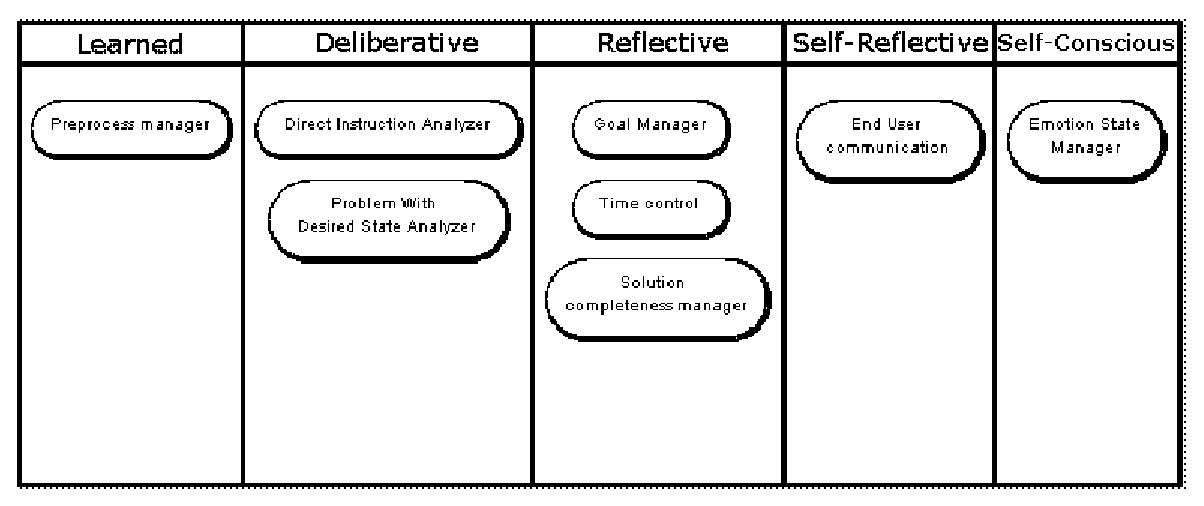
\epsfig{file=tuactivity5.eps, height=150px, width=340px}

\caption{Thinking Model Diagram}
\end{figure}

\subsection{Learned}

\subsubsection{Preprocess manager.} This manager activates several Way To Think to perform initial incident processing. The goal on this critic is to prepare and formalize incident description. There are several Way To Think:
\begin{itemize}
 \item Auto Correction of spelling
 \item Synonymic search
 \item Annotation – finding existing concepts in Knowledge Base
\end{itemize}

\subsection{Deliberative}

On the deliberative level selects suitable analyzers from Knowledge Base for Learned level, searches solutions.

\subsubsection{Direct Instruction Analyzer.} This Critic activates when direct instruction detected in incoming request. For example, “Please install MS Office 2012” is a direct instruction for system.
\subsubsection{Problem With Desired State Analyzer.} Critic activates when problem with desired state detected by the system. For example, “I have Internet Explorer 8 installed, but finance software required Internet Explorer 7”.

\subsection{Reflective}

On the reflective level system sets processing goals, performs time control, solution completeness manager.

\subsubsection{Goal manager.} Processing goals required to increase performance of incident processing. They have linked critics, way to think Main goal is a Help User. There are other goals, that derived from it, for example:
\begin{itemize}
 \item Resolve incident
 \item Understand incident type
 \item Model Direct Instruction
\end{itemize}
Goal manager links way to think with actions and finds required for selected goal processing way to think.

\subsubsection{Time control.} Time control watches across the thinking levels for time of incident processing. (SLA\footnote{SLA-Service Layer Agreement, the time for which incident should be processed} in terms of IS domain)

\subsubsection{Solution completeness manager.} This manager runs solution analysis to check if solution is completed.

\subsection{Self-reflective}
On this level system controls actions on lower levels like initialize Short Term Memory Context or starts time control. All communication of user is also regulated on this level by Do Not Understand Manager and communication with end user.\\
Practical example: System doesn't know concept "Opera software". Using the clarification request system learns new concept.

\subsubsection{Dialog mode.}
Important part of prototype implementation is an ability to work in Dialog mode with end user. When system faces with problem (e.g. unknown concept) it solves this issue asking help from human specialist.

\subsection{Self-conscious}
This level is a top in hierarchy. On this level system watches its Emotional State. By reacting for long incident processing system changes emotional state to allocate resources for processing.

\subsection{Training}
System trains while operation through the communication with human specialist. However, current prototype can work in separate training mode. In which system perceives all input data as training requests.

\section{Initial processing results}

\emph{TBD}

\section{Conclusions}

The main goal of described prototype is to demonstrate application of "Emotion Machine" \cite{minsk} in IT Maintenance Domain covering the cycle from incident in natural language end with understated request. (In future applied solution). Using the training ability prototype can evolute during the operation.

\begin{thebibliography}{4}

\bibitem{minsk}
Minsky M.:
The Emotion Machine.
Simon \& Schuster Paperbacks  (2006).

\bibitem{lili}
Liu H., Lieberman H.:
Metafor: Visualizing Stories as Code.
Cambridge, MIT Media Laboratory  (2005).

\bibitem{runo}
Russel S., Norvig P.:
Artificial Intelligence. A Modern approach.
Pearson (2010).

\end{thebibliography}

\end{document}

